% !TeX program = xelatex
\documentclass[UTF8,a4paper,12pt]{ctexart}

\usepackage[a4paper,margin=2.5cm]{geometry}
\usepackage{amsmath,amssymb}
\usepackage{booktabs}
\usepackage{tabularx}
\usepackage{array}
\usepackage{makecell}
\usepackage{multirow}
\usepackage{graphicx}
\usepackage{float}
\usepackage{xcolor}
\usepackage{enumitem}
\usepackage{hyperref}
\usepackage{caption}
\usepackage{subcaption}
\usepackage{tikz}
\usepackage{algorithm}
\usepackage{algpseudocode}
\usetikzlibrary{arrows.meta,positioning,fit,calc,shapes.geometric}

\hypersetup{
  colorlinks=true,
  linkcolor=blue,
  citecolor=blue,
  urlcolor=blue,
  pdftitle={面向 SMAC 任务的 Attention Residuals 迁移适配性实验研究},
  pdfauthor={刘少腾}
}

\setlist[itemize]{leftmargin=2em,itemsep=0.2em}
\setlist[enumerate]{leftmargin=2em,itemsep=0.2em}
\captionsetup{font=small,labelfont=bf}
\renewcommand{\arraystretch}{1.15}
\setlength{\emergencystretch}{3em}

\newcommand{\code}[1]{\texttt{#1}}

\title{面向 SMAC 任务的 Attention Residuals 迁移适配性实验研究}
\author{刘少腾}
\date{\today}

\begin{document}

\maketitle

\begin{abstract}
本文研究 Attention Residuals 从大语言模型结构到多智能体强化学习中的迁移适配性问题。
Attention Residuals 在深层语言模型中用于缓解 residual stream 中的信息稀释，但经典 PyMARL/SMAC 中的 recurrent agent 通常较浅，直接迁移该结构是否有效仍缺乏验证。
本文基于 PyMARL，在保持 QMIX、IQL、VDN 等算法主体不变的前提下，将 Attention Residuals 接入 RNN agent 的 hidden state 与 Q head 之间，并设计 Full、Lightweight、Block 以及 depth-only control 多种变体。
现有实验表明，重型 Full/Block AttnRes 直接迁移到浅层 MARL agent 后表现不稳定且训练成本较高；Lightweight AttnRes-L2 在部分指标上呈现 AUC 和 best-win 信号，但 final win rate 未稳定超过 baseline。
本文将当前结果定位为结构迁移适配性分析，而不是强算法性能主张，并进一步讨论将 selective attention 从 depth-wise residual transfer 转向 agent-wise communication 的后续研究方向。

\textbf{关键词：} 多智能体强化学习；SMAC；QMIX；Attention Residuals；结构迁移；注意力机制

\end{abstract}

\tableofcontents
\newpage

\section{引言}

\subsection{研究背景}

多智能体强化学习（multi-agent reinforcement learning, MARL）研究多个智能体在共享环境中通过交互学习协同行为的问题。
与单智能体强化学习相比，MARL 需要同时面对环境动态变化、智能体间策略相互影响以及局部观测条件下的协同决策。
在许多实际协同控制任务中，每个智能体只能获得自身附近的局部信息，却需要通过个体动作共同优化全局目标。
这种设定使得 MARL 不仅需要解决传统强化学习中的探索与长期回报估计问题，还需要处理智能体间的协调、信用分配以及非平稳训练目标等挑战。
\todo{补充 MARL、CTDE 和多智能体信用分配相关引用。}

集中训练、分散执行（centralized training with decentralized execution, CTDE）是协同 MARL 中常用的训练范式。
在该范式下，训练阶段可以利用全局状态或联合经验来稳定学习，而执行阶段每个智能体仍只依赖自身局部观测进行动作选择。
基于价值分解的方法是 CTDE 框架中的重要分支，其中 VDN 将联合动作价值函数表示为个体价值函数的加和，QMIX 进一步使用满足单调性约束的 mixing network 提升联合价值函数的表达能力。
IQL 则将多智能体问题拆分为多个独立 Q-learning 问题，虽然结构简单，但仍是评估新结构时常用的基础对照。
\todo{补充 IQL、VDN、QMIX 的正式引用。}

SMAC（StarCraft Multi-Agent Challenge）是评估协同 MARL 算法的经典 benchmark。
在 SMAC 中，每个智能体控制一个星际争霸 II 单位，并基于局部观测完成移动、攻击和集火等微操动作。
该环境能够较好地体现部分可观测、单位协同、异质智能体控制和探索路径敏感等问题，因此常被用于比较 QMIX、VDN、IQL 及其改进方法。
本文选择 SMAC 中的 \code{5m\_vs\_6m} 和 \code{3s5z} 作为主要实验地图：前者用于观察数量劣势下的同质单位协同，后者用于补充异质单位场景下的适配性分析。
\todo{补充 SMAC 官方论文引用，并确认地图 difficulty 标签。}

\subsection{LLM 结构迁移的动机}

近年来，大语言模型（large language models, LLMs）的快速发展推动了深层网络结构设计的持续演进。
在 Transformer 架构中，残差连接为深层模型提供了稳定的信息通道，使得模型可以在多层堆叠中保留和组合不同层次的表示。
然而，当网络深度不断增加时，固定形式的 residual accumulation 也可能带来信息混合和表示稀释问题：后续层接收到的是大量历史表示的累积结果，而这些历史表示并非总是对当前层同等重要。

Attention Residuals 针对这一问题提出了一种基于注意力的跨层信息选择机制。
其核心思想是，不再将残差流简单视为固定累加项，而是允许模型在 depth dimension 上对不同历史表示进行可学习的选择和聚合。
对于深层语言模型而言，这种机制有助于缓解 residual stream dilution，并增强模型对前层有用信息的选择能力。
\todo{补充 Attention Residuals 原论文及 residual stream analysis 相关引用。}

这一结构思想具有一定的迁移吸引力。
MARL 中的 recurrent agent 同样需要在有限表示维度中编码历史观测、局部状态和动作价值信息。
如果 depth-wise selective aggregation 能够改善 agent hidden representation，那么它可能为经典 PyMARL agent 提供一种低侵入式结构增强方式。
基于这一动机，本文尝试将 Attention Residuals 接入 RNN agent 的 hidden state 与 Q head 之间，在保持 QMIX、IQL、VDN 等算法主体不变的前提下，研究该结构是否能够迁移到 SMAC 多智能体强化学习任务中。

\subsection{迁移适配性问题}

尽管 Attention Residuals 在 LLM 中具有明确的结构动机，但直接迁移到 MARL 并不必然有效。
LLM 与经典 PyMARL agent 在网络深度、训练目标和任务瓶颈上均存在显著差异。
LLM 通常由大量 Transformer blocks 堆叠而成，residual stream 是跨层信息传递的主要通道；而 PyMARL 中常用的 RNN agent 结构较浅，通常可以概括为 \code{fc1 -> GRUCell -> fc2}。
因此，LLM 中的深层 residual dilution 问题并不会以相同形式出现在浅层 recurrent MARL agent 中。

另一方面，SMAC 任务的核心难点更多来自多智能体决策本身。
每个智能体只能基于局部观测行动，训练过程中还需要在非平稳的联合策略空间中学习稳定的价值估计。
对于 QMIX 等价值分解方法而言，个体价值函数和全局价值函数之间的关系、探索过程中产生的轨迹分布以及不同智能体之间的隐式协同，往往比单个 agent 内部的网络深度更关键。
在这种背景下，将 LLM 中用于深层残差信息选择的模块直接放在 GRU hidden state 后面，可能会引入额外参数和训练方差，却未必能作用于 MARL 的主要瓶颈。

因此，本文将 Attention Residuals 到 MARL 的迁移视为一个适配性分析问题，而不是预设其必然带来性能提升。
具体而言，本文关注两类结构错位：第一，原始 Attention Residuals 面向深层 Transformer residual stream，而本文所用 PyMARL agent 是浅层 recurrent network；第二，LLM 中 attention residual 强调跨层信息选择，而 SMAC 中更自然的 attention 使用场景可能是智能体间通信和交互建模。
这种区分对于理解实验结果十分重要，也为后续从 depth-wise residual transfer 转向 agent-wise attention communication 提供了动机。

\subsection{研究问题与贡献}

围绕上述迁移动机和结构错位，本文主要回答以下三个研究问题。

第一，直接将 Attention Residuals 插入 \code{GRU hidden -> Q head} 之间，是否能够在 SMAC 任务中稳定提升学习效果？
为回答该问题，本文在 QMIX 上构建 Full AttnRes 和 Block AttnRes 两种重型直接迁移版本，并在 \code{5m\_vs\_6m} 与 \code{3s5z} 上进行多 seed 对比。

第二，轻量化 Attention Residuals 是否比重型结构更适合浅层 recurrent agent？
考虑到 PyMARL agent 的网络深度和表示维度较小，本文进一步设计 AttnRes-L2 轻量化变体，用于观察降低结构复杂度后是否能够获得更稳定的学习信号。

第三，性能变化是否仅仅来自额外网络深度？
为避免将“网络变深”误判为 Attention Residuals 的作用，本文加入 depth-only control，即只增加 residual MLP stack，而不使用 attention、learnable query 或 depth-wise selection。
该对照有助于区分选择性聚合机制与单纯增加参数量之间的影响。

本文的贡献可以概括为三点。
首先，本文在 PyMARL 框架中实现了 Attention Residuals 到 recurrent MARL agent 的迁移，并保持 QMIX、IQL 和 VDN 等算法主体不变，从而使实验聚焦于 agent 侧结构适配问题。
其次，本文系统比较 Full、Lightweight、Block 和 depth-only control 多类变体，在 \code{5m\_vs\_6m} 与 \code{3s5z} 上分析其 final win rate、best win rate、AUC 和训练时间。
已有结果表明，重型 Full/Block AttnRes 直接迁移并不稳定且成本较高，Lightweight AttnRes-L2 在部分 AUC 和 best-win 指标上显示出有限信号，但尚不能支持稳定优于 baseline 的强结论。
最后，本文基于实验现象讨论 LLM 结构与 MARL 任务瓶颈之间的错位，并提出将 selective attention 从 depth-wise residual transfer 转向 agent-wise communication 的后续研究方向。

需要强调的是，本文并不主张当前 AttnRes-RNN 是一个优于 QMIX 的强算法。
相反，本文的目标是通过系统实验说明：直接迁移 LLM 中用于深层残差信息流的结构到浅层 MARL agent 时，需要谨慎分析其适配性、训练成本和任务瓶颈是否匹配。

\section{相关工作}

\subsection{多智能体强化学习与价值分解}

多智能体强化学习关注多个智能体在共享环境中通过交互学习策略的问题。
在完全协作任务中，所有智能体通常共享同一个团队回报，但每个智能体只能基于自身局部观测进行动作选择。
这种设定会带来两个核心困难：一方面，单个智能体无法直接观测完整环境状态；另一方面，团队回报难以明确分配给每个智能体的局部动作。
因此，如何在训练阶段利用更多全局信息，同时在执行阶段保持分散决策，是协同 MARL 方法长期关注的问题。
CTDE、集中式 critic 和多智能体信用分配方法为这一方向提供了常用建模框架 \cite{oliehoek2016concise,lowe2017multiagent,foerster2018counterfactual}。

集中训练、分散执行（CTDE）为这一问题提供了常用范式。
在训练阶段，算法可以使用全局状态、联合动作或其他智能体信息来估计价值函数；在执行阶段，每个智能体仍只使用局部观测独立决策。
价值分解方法是 CTDE 中的重要路线，其基本思想是学习个体 action-value，并通过某种分解或混合方式得到联合 action-value。
这种方式兼顾了分散执行的需求和集中训练的稳定性，因此成为 SMAC 等协同控制任务中的常用基线。

IQL、VDN 和 QMIX 是本文涉及的三类代表性方法。
IQL 将多智能体问题拆分为多个独立 Q-learning 问题，结构简单，能够作为判断新 agent 结构是否具有泛化信号的基础对照。
VDN 假设联合价值函数可以表示为个体价值函数之和，从而实现简单而可解释的价值分解。
QMIX 在 VDN 的基础上引入单调 mixing network，允许联合价值函数以更灵活的方式依赖全局状态，同时保持个体 greedy action 与联合 greedy action 的一致性。
这些方法分别代表独立价值学习、加性价值分解和单调价值混合三类典型设置 \cite{tan1993multiagent,sunehag2018value,rashid2018qmix}。

本文选择这些方法并不是为了提出一个新的价值分解框架，而是为了隔离分析 agent 侧结构迁移的影响。
具体而言，本文保持 learner、mixer、探索策略和训练流程尽量不变，只在 recurrent agent 的 hidden representation 后接入 Attention Residuals 或 depth-only control。
这种设计使实验更聚焦于一个问题：源自 LLM 的 residual attention 结构是否适合作为浅层 MARL agent 的表征后处理模块。

\subsection{SMAC 与协同控制任务}

SMAC（StarCraft Multi-Agent Challenge）是评估协同 MARL 算法的经典实验环境。
该环境将星际争霸 II 中的单位微操任务抽象为多智能体控制问题，每个智能体控制一个己方单位，并在局部观测条件下选择移动、攻击、停止等离散动作。
由于智能体无法直接获得完整敌我状态，且每个单位的动作会影响团队整体战斗结果，SMAC 能够较好地反映部分可观测、协同决策和信用分配等问题。
SMAC 因此成为评估协作型 MARL 方法的常用 benchmark \cite{samvelyan2019starcraft}。

与许多单智能体控制任务相比，SMAC 的难点不仅在于学习有效的动作价值估计，还在于不同智能体之间需要形成隐式协作。
例如，在数量劣势地图中，智能体需要学会集火、拉扯和避免无效攻击；在异质单位地图中，不同单位类型的攻击范围、生命值和移动能力不同，策略需要体现角色分工。
因此，SMAC 不仅适合比较最终胜率，也适合观察不同算法在学习速度、seed 方差和训练稳定性方面的差异。

本文选择 \code{5m\_vs\_6m} 和 \code{3s5z} 作为主要分析地图。
\code{5m\_vs\_6m} 是同质 Marine 对抗地图，敌方比己方多一个单位，因此对集中火力、局部走位和探索路径较敏感，适合作为区分不同结构适配性的主要诊断任务。
\code{3s5z} 包含不同类型单位，更能体现异质 agent 协同，但在本文实验设置下多数方法接近较高胜率，因此更适合作为辅助 sanity check，而不是单独支撑强结论的地图。
具体而言，\code{3s5z} 是 3 个 Stalkers 与 5 个 Zealots 对抗相同敌方编队的 easy 场景。

\subsection{注意力机制在 MARL 中的应用}

注意力机制已经被广泛用于建模序列、集合和图结构中的选择性信息聚合。
在 MARL 场景中，attention 的一个自然用途是建模智能体之间的交互关系。
由于每个智能体的决策通常只依赖局部观测，若能够通过 attention 从其他智能体的状态、隐藏表示或消息中选择有用信息，就可能缓解部分可观测条件下的协同困难。
例如，基于注意力的 actor-critic 和通信方法已经被用于学习智能体间的选择性信息聚合 \cite{iqbal2019actor,das2019tarmac}。

已有 MARL attention 方法通常关注 agent-wise interaction 或 communication。
这类方法可以让每个智能体根据自身 hidden state 对其他智能体表示进行加权聚合，从而形成与当前决策相关的通信消息。
也有工作将智能体视为图节点，使用 graph attention 或 transformer-style encoder 建模智能体间关系。
这些方法的共同点是将 attention 用于跨智能体信息选择，其目标直接对应 MARL 中的协同与交互问题。
图神经网络和 Transformer 风格方法进一步将这种思想扩展到动态交互图和序列化多智能体决策中 \cite{jiang2020graph,wen2022multiagenttransformer}。

本文主实验与上述工作存在重要差异。
本文首先尝试将 LLM 中的 Attention Residuals 迁移为 agent 内部的 depth-wise residual aggregation 模块，而不是直接采用已有的跨智能体 attention 算法。
换言之，本文主线关注的是“跨层表示选择”能否作为 recurrent agent 的后处理增强。
在后半部分，本文进一步基于 direct depth-wise transfer 的不稳定结果，引入 AttnComm-QMIX-L2 作为 agent-wise communication 扩展，用于验证 selective attention 是否在更贴近 MARL 协同瓶颈的位置产生更清晰的正向信号。

\subsection{残差连接与深层网络信息流}

残差连接最初被用于缓解深层神经网络训练困难，使网络可以通过恒等映射更稳定地传播梯度和表示。
在 Transformer 架构中，残差连接进一步成为层间信息流的核心通道。
对于深层模型而言，残差流不仅承担优化上的作用，也承担表示组合的作用：后续层在前序层表示基础上持续更新特征，并通过多层堆叠形成更复杂的语义抽象。
ResNet 与 Transformer 的成功说明，稳定的跨层信息通道是深层网络训练中的关键结构之一 \cite{he2016deep,vaswani2017attention}。

随着语言模型深度增加，固定 residual accumulation 也可能带来新的问题。
如果每一层都将自身输出写入同一 residual stream，后续层接收到的表示会包含大量历史信息，而这些信息对当前计算并不总是同等重要。
这种现象可以被理解为 residual stream 中的信息稀释或无选择累积。
因此，如何让模型在深层网络中更有选择地利用前层表示，成为改进 LLM 架构的一类重要问题。
预归一化 Transformer 的稳定性分析也表明，归一化位置和残差路径会显著影响深层模型的优化行为 \cite{xiong2020layernorm}。

Attention Residuals 针对上述问题提出了基于 attention 的 depth-wise selection。
其基本思想是让后续层不再被动接收固定累加的 residual，而是通过可学习 query 对不同 depth source 进行加权选择。
这种设计与 Dense connection、skip connection、cross-layer aggregation 等思想在目标上相关，都是为了改善深层网络中的信息流动。
不同之处在于，Attention Residuals 强调使用 attention 机制进行动态选择，而不是预先固定跨层连接方式。
本文以 Attention Residuals 的公开技术报告作为结构迁移来源 \cite{kimi2026attentionresiduals}。

本文借鉴的是 Attention Residuals 中“选择性聚合”的结构思想。
然而，本文并不直接假设该机制在 MARL 中会产生与 LLM 相同的收益。
由于 PyMARL agent 通常较浅，depth-wise residual dilution 可能并不是主要瓶颈，因此本文需要通过 full、lightweight、block 和 depth-only control 等变体实验来判断这一结构思想是否适配。

\subsection{LLM 结构向强化学习迁移}

近年来，Transformer 和大模型结构逐渐被引入强化学习。
一类工作将轨迹建模为序列，并使用 Transformer 进行行为建模或决策生成；另一类工作则尝试将 attention、残差连接、归一化和大模型训练经验迁移到策略网络或价值网络中。
这些工作说明，LLM 或 Transformer 中的结构经验可能为强化学习提供新的模型设计启发。
例如，Decision Transformer 将离线强化学习轨迹建模为序列预测问题，展示了 Transformer 结构在决策建模中的潜力 \cite{chen2021decisiontransformer}。

不过，结构迁移并不等价于直接复用模块。
强化学习训练目标通常具有非平稳、bootstrapping 和探索分布变化等特点，价值学习中的误差传播也可能使额外网络结构带来更高方差。
在 MARL 中，这些问题还会与多智能体非平稳性和信用分配进一步叠加。
因此，一个在监督式语言建模中有效的结构，并不必然能在 MARL 中以相同方式发挥作用。

本文与已有 LLM-to-RL 迁移工作的区别在于，本文重点不是提出一个追求最优性能的新 MARL 算法，而是研究一个具体结构思想的适配边界。
Attention Residuals 的原始动机来自深层 LLM 的 residual stream，而本文实验对象是浅层 recurrent MARL agent。
这种结构和任务之间的差异，使得本文更关注“迁移是否合理、在哪些设置下有信号、何时应止损”。

从这一角度看，本文的实验结果即使不是单纯正向，也具有分析价值。
如果重型 depth-wise AttnRes 直接迁移表现不稳定，而轻量化版本只在部分指标上有有限信号，那么结论不应被表述为算法失败，而应被理解为结构迁移中的适配性证据。
这也为后续将 selective attention 重新放置到 agent communication 维度提供了理论和实验动机。

\section{实验环境与基线方法}

\subsection{SMAC 环境与 MARL 问题定义}

本文实验基于 SMAC 环境。
每个 agent 控制一个己方单位，根据局部观测选择离散动作，包括移动、停止和攻击敌方单位等。
训练过程中使用 PyMARL 默认的 shaped reward，并在测试阶段统计 battle won rate。

从多智能体强化学习角度看，SMAC 可以形式化为一个 Dec-POMDP：
\begin{equation}
  \mathcal{G} =
  \langle \mathcal{S}, \mathcal{U}, P, r, \mathcal{Z}, O, n, \gamma \rangle ,
\end{equation}
其中 \(\mathcal{S}\) 表示全局状态空间，\(\mathcal{U}\) 表示单个智能体动作空间，\(n\) 为智能体数量，\(P\) 为状态转移函数，\(r\) 为团队共享奖励，\(\mathcal{Z}\) 为局部观测空间，\(O\) 为观测函数，\(\gamma\) 为折扣因子。
在时刻 \(t\)，第 \(i\) 个智能体获得局部观测 \(o_i^t \in \mathcal{Z}\)，根据自身历史轨迹 \(\tau_i^t\) 选择动作 \(u_i^t \in \mathcal{U}\)。
联合动作记为 \(\mathbf{u}^t=(u_1^t,\ldots,u_n^t)\)，团队目标是最大化折扣回报：
\begin{equation}
  J(\pi)=
  \mathbb{E}_{\pi}
  \left[
    \sum_{t=0}^{\infty} \gamma^t r_t
  \right],
\end{equation}
其中分散执行策略通常写为
\begin{equation}
  \pi(\mathbf{u}^t \mid \boldsymbol{\tau}^t)
  =
  \prod_{i=1}^{n}
  \pi_i(u_i^t \mid \tau_i^t).
\end{equation}

\begin{table}[H]
  \centering
  \caption{实验地图信息}
  \label{tab:maps}
  \begin{tabularx}{\linewidth}{llllX}
    \toprule
    地图 & 己方单位 & 敌方单位 & 类型 & 作用 \\
    \midrule
    \code{5m\_vs\_6m} & 5 Marines & 6 Marines & 同质单位 & 主要诊断地图，用于测试数量劣势下的协同、集火和走位。 \\
    \code{3s5z} & 3 Stalkers + 5 Zealots & 3 Stalkers + 5 Zealots & 异质单位 & 辅助地图，用于测试混合单位协同；当前结果接近饱和。 \\
    \bottomrule
  \end{tabularx}
\end{table}

按照 SMAC 地图设定，\code{5m\_vs\_6m} 通常被归为 hard 场景，\code{3s5z} 为 symmetric heterogeneous easy 场景。

\subsection{Recurrent Agent 与独立价值学习}

PyMARL 中常用的 agent 是一个共享参数的 recurrent Q-network。
对第 \(i\) 个智能体，输入 \(x_i^t\) 通常由局部观测、上一时刻动作和 agent id 拼接得到。
本文基线 agent 的计算过程为：
\begin{align}
  e_i^t &= \mathrm{ReLU}(W_e x_i^t+b_e), \\
  h_i^t &= \mathrm{GRUCell}(e_i^t, h_i^{t-1}), \\
  Q_i^t &= W_q h_i^t+b_q ,
\end{align}
其中 \(h_i^t\) 是智能体隐藏状态，\(Q_i^t \in \mathbb{R}^{|\mathcal{U}|}\) 是该智能体对所有离散动作的 action-value 输出。

IQL 将每个智能体视作独立 Q-learning 问题。
对单个智能体，TD target 可写为：
\begin{equation}
  y_i^t =
  r_t + \gamma
  \max_{u_i'}
  Q_i^{-}(\tau_i^{t+1}, u_i'),
\end{equation}
对应 TD loss 为：
\begin{equation}
  \mathcal{L}_{\mathrm{IQL}}(\theta)
  =
  \mathbb{E}
  \left[
    \left(
      y_i^t - Q_i(\tau_i^t,u_i^t;\theta)
    \right)^2
  \right].
\end{equation}
由于 IQL 不显式建模联合动作价值函数，它结构简单，但容易受到多智能体非平稳性影响。

\subsection{VDN 与 QMIX 价值分解}

VDN 假设联合动作价值函数可以由个体动作价值函数加和得到：
\begin{equation}
  Q_{\mathrm{tot}}(\boldsymbol{\tau},\mathbf{u})
  =
  \sum_{i=1}^{n} Q_i(\tau_i,u_i).
\end{equation}
该形式简单且便于分散执行，但表达能力受限，因为所有智能体对联合价值的贡献被限制为线性相加。

QMIX 使用 mixing network 将个体 \(Q_i\) 混合为联合动作价值：
\begin{equation}
  Q_{\mathrm{tot}}(\boldsymbol{\tau},\mathbf{u},s)
  =
  f_{\mathrm{mix}}
  \left(
    Q_1(\tau_1,u_1),\ldots,Q_n(\tau_n,u_n),s
  \right),
\end{equation}
并要求满足单调性约束：
\begin{equation}
  \frac{\partial Q_{\mathrm{tot}}}{\partial Q_i} \ge 0,
  \quad
  \forall i \in \{1,\ldots,n\}.
\end{equation}
该约束保证联合 greedy action 可以通过每个智能体局部 greedy action 得到，从而兼顾集中训练和分散执行。

对 VDN 和 QMIX，联合 TD target 可写为：
\begin{equation}
  y_{\mathrm{tot}}^t =
  r_t + \gamma
  Q_{\mathrm{tot}}^{-}
  \left(
    \boldsymbol{\tau}^{t+1},
    \mathbf{u}^{*},
    s^{t+1}
  \right),
\end{equation}
其中 \(\mathbf{u}^{*}\) 由 target agent 或 double Q-learning 选择。
训练目标为：
\begin{equation}
  \mathcal{L}_{\mathrm{TD}}(\theta)
  =
  \mathbb{E}
  \left[
    \left(
      y_{\mathrm{tot}}^t -
      Q_{\mathrm{tot}}(\boldsymbol{\tau}^{t},\mathbf{u}^{t},s^{t};\theta)
    \right)^2
  \right].
\end{equation}

\begin{figure}[H]
  \centering
  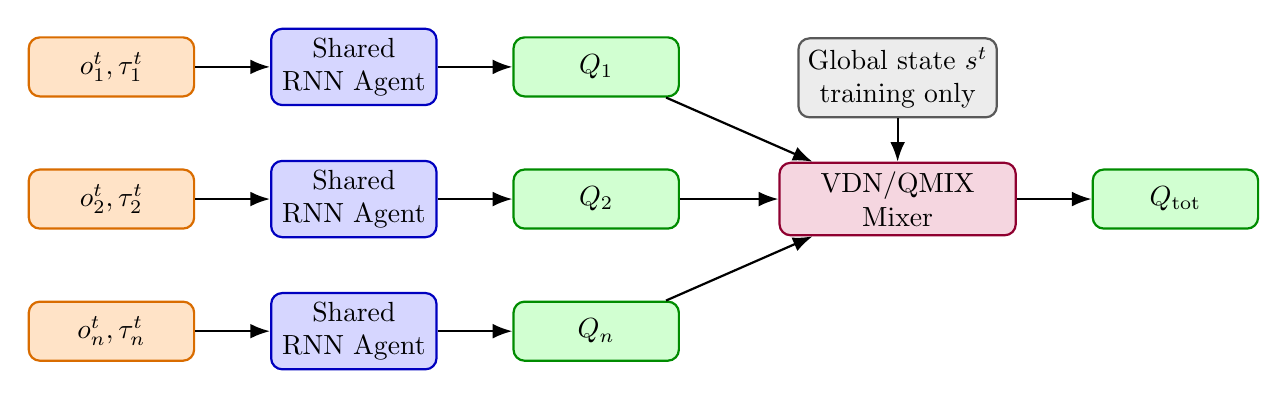
\begin{tikzpicture}[
    node distance=0.9cm and 0.95cm,
    box/.style={draw, rounded corners, thick, minimum width=2.1cm, minimum height=0.75cm, align=center},
    obs/.style={box, fill=orange!22, draw=orange!85!black},
    agent/.style={box, fill=blue!16, draw=blue!75!black},
    qval/.style={box, fill=green!18, draw=green!55!black},
    mixer/.style={box, fill=purple!16, draw=purple!75!black, minimum width=3.0cm},
    state/.style={box, fill=gray!15, draw=gray!70!black},
    arr/.style={-{Latex[length=2.5mm]}, thick}
  ]
    \node[obs] (o1) {\(o_1^t,\tau_1^t\)};
    \node[obs, below=of o1] (o2) {\(o_2^t,\tau_2^t\)};
    \node[obs, below=of o2] (on) {\(o_n^t,\tau_n^t\)};

    \node[agent, right=of o1] (a1) {Shared\\RNN Agent};
    \node[agent, right=of o2] (a2) {Shared\\RNN Agent};
    \node[agent, right=of on] (an) {Shared\\RNN Agent};

    \node[qval, right=of a1] (q1) {\(Q_1\)};
    \node[qval, right=of a2] (q2) {\(Q_2\)};
    \node[qval, right=of an] (qn) {\(Q_n\)};

    \node[mixer, right=1.25cm of q2] (mix) {VDN/QMIX\\Mixer};
    \node[state, above=0.55cm of mix] (s) {Global state \(s^t\)\\training only};
    \node[qval, right=of mix] (qt) {\(Q_{\mathrm{tot}}\)};

    \draw[arr] (o1) -- (a1);
    \draw[arr] (o2) -- (a2);
    \draw[arr] (on) -- (an);
    \draw[arr] (a1) -- (q1);
    \draw[arr] (a2) -- (q2);
    \draw[arr] (an) -- (qn);
    \draw[arr] (q1) -- (mix);
    \draw[arr] (q2) -- (mix);
    \draw[arr] (qn) -- (mix);
    \draw[arr] (s) -- (mix);
    \draw[arr] (mix) -- (qt);
  \end{tikzpicture}
  \caption{PyMARL 中基于价值分解的训练框架示意。多个智能体共享 RNN agent 参数，输出个体动作价值，VDN/QMIX mixer 在训练阶段生成联合动作价值。}
  \label{fig:pymarl-qmix-framework}
\end{figure}

\subsection{评价指标}

本文使用以下指标评估模型性能。
设第 \(k\) 次测试发生在训练步 \(t_k\)，测试胜率为 \(w_k\)，测试回报为 \(R_k\)。
final test win rate 表示训练结束附近的测试胜率；best test win rate 表示训练过程中的最高测试胜率：
\begin{equation}
  w_{\mathrm{best}} = \max_k w_k.
\end{equation}
win-rate AUC 用于衡量整个训练过程中的学习质量：
\begin{equation}
  \mathrm{AUC}
  =
  \frac{1}{t_K-t_1}
  \sum_{k=1}^{K-1}
  \frac{w_k+w_{k+1}}{2}
  (t_{k+1}-t_k).
\end{equation}
此外，本文还报告 final test return、wall-clock hours 和 paired seed delta，用于分析最终性能、训练成本和 seed 稳定性。

\section{Attention Residuals 的 MARL 适配方法}

\subsection{总体结构}

本文保持 QMIX、IQL、VDN 的 learner、mixer 和训练流程不变，只修改 agent 网络。
原始 RNN agent 首先将输入编码为 hidden state，再直接通过 Q head 输出动作价值：
\begin{align}
  e_i^t &= \mathrm{ReLU}(W_e x_i^t+b_e), \\
  h_i^t &= \mathrm{GRUCell}(e_i^t,h_i^{t-1}), \\
  Q_i^t &= W_q h_i^t + b_q.
\end{align}

AttnRes-RNN agent 在 GRU hidden state 与 Q head 之间加入 Depthwise Attention Residual 模块：
\begin{align}
  \bar{h}_i^t &= \mathrm{AttnRes}(h_i^t), \\
  Q_i^t &= W_q \bar{h}_i^t + b_q.
\end{align}
Depth-only control 则将该模块替换为普通 residual MLP stack，用于判断性能变化是否只是来自额外网络深度。

\begin{figure}[H]
  \centering
  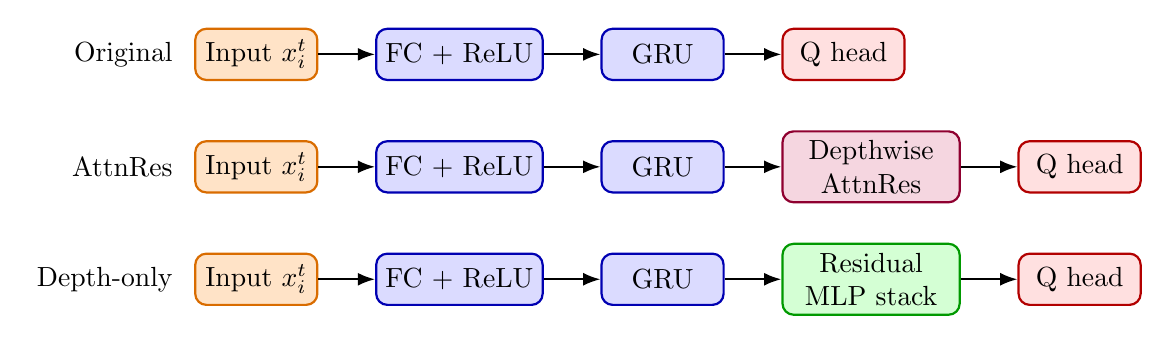
\begin{tikzpicture}[
    node distance=0.65cm and 0.72cm,
    block/.style={draw, rounded corners, thick, minimum width=1.55cm, minimum height=0.65cm, align=center},
    input/.style={block, fill=orange!22, draw=orange!85!black},
    core/.style={block, fill=blue!14, draw=blue!70!black},
    attn/.style={block, fill=purple!16, draw=purple!75!black, minimum width=2.25cm},
    mlp/.style={block, fill=green!17, draw=green!60!black, minimum width=2.25cm},
    qout/.style={block, fill=red!12, draw=red!70!black},
    arr/.style={-{Latex[length=2.2mm]}, thick}
  ]
    \node[input] (x1) {Input \(x_i^t\)};
    \node[core, right=of x1] (fc11) {FC + ReLU};
    \node[core, right=of fc11] (gru1) {GRU};
    \node[qout, right=of gru1] (q1) {Q head};
    \node[left=0.15cm of x1] (l1) {Original};
    \draw[arr] (x1) -- (fc11);
    \draw[arr] (fc11) -- (gru1);
    \draw[arr] (gru1) -- (q1);

    \node[input, below=0.75cm of x1] (x2) {Input \(x_i^t\)};
    \node[core, right=of x2] (fc12) {FC + ReLU};
    \node[core, right=of fc12] (gru2) {GRU};
    \node[attn, right=of gru2] (ar) {Depthwise\\AttnRes};
    \node[qout, right=of ar] (q2) {Q head};
    \node[left=0.15cm of x2] (l2) {AttnRes};
    \draw[arr] (x2) -- (fc12);
    \draw[arr] (fc12) -- (gru2);
    \draw[arr] (gru2) -- (ar);
    \draw[arr] (ar) -- (q2);

    \node[input, below=0.75cm of x2] (x3) {Input \(x_i^t\)};
    \node[core, right=of x3] (fc13) {FC + ReLU};
    \node[core, right=of fc13] (gru3) {GRU};
    \node[mlp, right=of gru3] (dm) {Residual\\MLP stack};
    \node[qout, right=of dm] (q3) {Q head};
    \node[left=0.15cm of x3] (l3) {Depth-only};
    \draw[arr] (x3) -- (fc13);
    \draw[arr] (fc13) -- (gru3);
    \draw[arr] (gru3) -- (dm);
    \draw[arr] (dm) -- (q3);
  \end{tikzpicture}
  \caption{原始 RNN agent、AttnRes-RNN agent 与 depth-only control 的结构对比。本文只修改 GRU hidden state 后的 agent 侧模块，保持 MARL 后端算法不变。}
  \label{fig:agent-structure}
\end{figure}

\subsection{Depthwise Attention Residual}

Depthwise Attention Residual 将 GRU hidden state 视作初始 depth source，并通过若干虚拟深度层生成新的 source。
设输入 hidden state 为 \(h \in \mathbb{R}^{d}\)，初始 source 集合为：
\begin{equation}
  \mathcal{S}_0 = \{h\}.
\end{equation}
第 \(\ell\) 个 AttnRes layer 使用一个可学习 query \(q_\ell \in \mathbb{R}^{d}\) 对当前 source 集合进行 attention：
\begin{align}
  \alpha_{\ell,j}
  &=
  \frac{
    \exp\left(q_\ell^{\top}\mathrm{RMSNorm}(s_j)/\sqrt{d}\right)
  }{
    \sum_{s_m\in\mathcal{S}_{\ell}}
    \exp\left(q_\ell^{\top}\mathrm{RMSNorm}(s_m)/\sqrt{d}\right)
  }, \\
  a_\ell
  &=
  \sum_{s_j\in\mathcal{S}_{\ell}}
  \alpha_{\ell,j}s_j .
\end{align}
随后，\(a_\ell\) 经过两层 MLP transform 得到新增 source：
\begin{align}
  u_\ell &= \mathrm{Dropout}\left(F_\ell(a_\ell)\right), \\
  \mathcal{S}_{\ell+1} &= \mathcal{S}_{\ell} \cup \{u_\ell\}, \\
  z_\ell &= a_\ell + u_\ell .
\end{align}
其中 \(z_\ell\) 是第 \(\ell\) 层输出，最终 AttnRes 模块返回 \(z_L\)。
在实现中，query 采用零初始化，以降低训练早期对原始 hidden representation 的扰动。

\subsection{Full、Lightweight 与 Block 变体}

Full AttnRes 使用上述完整 depth-wise attention 过程，并在本文实验中设置 \(L=4\)。
它对应最直接的重型结构迁移，即在浅层 recurrent agent 后额外构造 4 层虚拟 depth source，并让每层都可以从所有已有 source 中选择信息。

Lightweight AttnRes-L2 与 Full AttnRes 使用相同公式，但将层数减少为 \(L=2\)。
该变体用于检验降低结构复杂度后，Attention Residuals 是否更适合 PyMARL 中较浅的 RNN agent。
如果 L2 版本相比 full 版本更稳定，则说明直接迁移重型 LLM 模块可能存在过度复杂化问题。

Block AttnRes 使用 block-wise source aggregation。
设 block size 为 \(B\)，每个 block 内部的新增 source 先累积为 partial block：
\begin{equation}
  p_{\ell} =
  \begin{cases}
    u_\ell, & \ell \text{ is the first layer in a block},\\
    p_{\ell-1}+u_\ell, & \text{otherwise}.
  \end{cases}
\end{equation}
当到达 block 边界时，\(p_\ell\) 被加入 completed block 集合；后续 attention 只在 completed blocks 和当前 partial block 上执行。
本文使用 \(L=4, B=2\) 的 block 设置，用于观察分块聚合是否能够改善 full 版本的稳定性。

\subsection{Depth-only Control}

Depth-only control 不使用 query、attention 或 RMSNorm，而是仅在 GRU hidden state 后添加 residual MLP stack。
设 \(z_0=P_{\mathrm{in}}h\)，则第 \(\ell\) 层计算为：
\begin{equation}
  z_\ell =
  \mathrm{ReLU}
  \left(
    z_{\ell-1}+G_\ell(z_{\ell-1})
  \right),
  \quad \ell=1,\ldots,L,
\end{equation}
最终输出为：
\begin{equation}
  \bar{h}=P_{\mathrm{out}}z_L.
\end{equation}
该对照组的作用是区分“额外深度”与“depth-wise attention selection”。
如果 depth-only control 不能稳定提升性能，则说明单纯增加后处理 MLP 深度并不是收益来源。

\begin{algorithm}[H]
  \caption{AttnRes-RNN Agent Forward Pass}
  \label{alg:attnres-rnn-forward}
  \begin{algorithmic}[1]
    \Require agent input \(x_i^t\), previous hidden state \(h_i^{t-1}\), AttnRes layers \(L\)
    \State \(e_i^t \gets \mathrm{ReLU}(W_e x_i^t+b_e)\)
    \State \(h_i^t \gets \mathrm{GRUCell}(e_i^t,h_i^{t-1})\)
    \State \(\mathcal{S} \gets \{h_i^t\}\)
    \For{\(\ell=1\) to \(L\)}
      \State \(a_\ell \gets \sum_{s_j\in\mathcal{S}}\mathrm{softmax}_j(q_\ell^\top \mathrm{RMSNorm}(s_j)/\sqrt{d})s_j\)
      \State \(u_\ell \gets \mathrm{Dropout}(F_\ell(a_\ell))\)
      \State \(\mathcal{S} \gets \mathcal{S} \cup \{u_\ell\}\)
      \State \(z_\ell \gets a_\ell+u_\ell\)
    \EndFor
    \State \(Q_i^t \gets W_q z_L+b_q\)
    \State \Return \(Q_i^t, h_i^t\)
  \end{algorithmic}
\end{algorithm}

\subsection{方法差异总结}

\begin{table}[H]
  \centering
  \caption{模型变体与实验目的}
  \label{tab:variants}
  \begin{tabularx}{\linewidth}{l l X l l}
    \toprule
    变体 & 基线算法 & Agent 修改 & 层数 & 目的 \\
    \midrule
    \code{qmix} & QMIX & 原始 RNN agent & - & baseline \\
    \code{qmix\_attnres} & QMIX & GRU 后接 Full AttnRes & 4 & 重型直接迁移 \\
    \code{qmix\_attnres\_l2} & QMIX & GRU 后接 Full AttnRes & 2 & 轻量化迁移 \\
    \code{qmix\_attnres\_block} & QMIX & GRU 后接 Block AttnRes & 4 & block-wise 迁移 \\
    \code{qmix\_depth\_mlp} & QMIX & GRU 后接 residual MLP stack & 4 & depth-only control \\
    \code{iql\_attnres\_l2} & IQL & GRU 后接轻量 AttnRes & 2 & 跨算法验证 \\
    \code{vdn\_attnres\_l2} & VDN & GRU 后接轻量 AttnRes & 2 & 跨算法验证 \\
    \bottomrule
  \end{tabularx}
\end{table}

本文所有变体均保持训练流程、环境设置和后端 MARL 算法尽量一致。
因此，实验结果主要反映 GRU 后处理模块对学习稳定性、样本效率和训练成本的影响。

\section{实验设置}

\subsection{训练配置}

实验基于 PyMARL 和 SMAC。
所有主实验均训练到相同的 \code{t\_max=2050000}，测试时使用 \code{test\_nepisode=32}，并在 seed 1、2、3 上重复。

\begin{table}[H]
  \centering
  \caption{主要训练超参数}
  \label{tab:hyperparams}
  \begin{tabularx}{0.82\linewidth}{l l X}
    \toprule
    超参数 & 取值 & 说明 \\
    \midrule
    \code{lr} & 0.0005 & 学习率 \\
    \code{batch\_size} & 32 & replay batch size \\
    \code{buffer\_size} & 5000 & episode replay buffer \\
    \code{epsilon\_start} & 1.0 & 初始探索率 \\
    \code{epsilon\_finish} & 0.05 & 最终探索率 \\
    \code{epsilon\_anneal\_time} & 50000 & epsilon 衰减步数 \\
    \code{target\_update\_interval} & 200 & target network 更新间隔 \\
    \code{mixing\_embed\_dim} & 32 & QMIX mixer hidden size \\
    \code{hypernet\_layers} & 2 & QMIX hypernetwork 层数 \\
    \code{hypernet\_embed} & 64 & QMIX hypernetwork hidden size \\
    \code{t\_max} & 2050000 & 训练步数上限 \\
    \code{test\_nepisode} & 32 & 每次测试 episode 数 \\
    \code{seeds} & 1,2,3 & 重复实验随机种子 \\
    \bottomrule
  \end{tabularx}
\end{table}

\subsection{实验分组}

QMIX 主线在 \code{5m\_vs\_6m} 和 \code{3s5z} 两张地图上比较五种变体。
跨算法验证在 \code{5m\_vs\_6m} 上比较 lightweight AttnRes-L2 与对应 baseline。

\begin{itemize}
  \item 主线：QMIX baseline、Full AttnRes、AttnRes-L2、Block AttnRes 与 depth-only control。
  \item 跨算法：IQL、VDN、QMIX baseline 与对应 AttnRes-L2 变体。
  \item 当前所有预设 paired comparison 均已补齐 3 个 seeds；VDN baseline 使用本地同步后的 Sacred run 100、101、102。
\end{itemize}

\subsection{日志与统计}

训练日志来自 Sacred 输出，汇总文件位于 \code{pymarl-results/diagnostics}。
本文使用 paired seed 方式比较同一算法 baseline 与 AttnRes-L2 candidate 的差异，并报告 final win、best win、win-rate AUC 和 wall-clock time。

\section{实验结果与分析}

\subsection{QMIX 主实验结果}

\begin{table}[H]
  \centering
  \caption{QMIX 主实验结果}
  \label{tab:qmix-main-results}
  \resizebox{\linewidth}{!}{
  \begin{tabular}{llrrrrr}
    \toprule
    地图 & 变体 & Seeds & Final Win & Best Win & Win AUC & Wall Hours \\
    \midrule
    \code{5m\_vs\_6m} & \code{qmix} & 3/3 & 0.6250 & 0.7813 & 0.3926 & 6.59 \\
    \code{5m\_vs\_6m} & \code{qmix\_attnres} & 3/3 & 0.5417 & 0.7188 & 0.4111 & 15.14 \\
    \code{5m\_vs\_6m} & \code{qmix\_attnres\_l2} & 3/3 & 0.6042 & 0.8021 & 0.4493 & 8.29 \\
    \code{5m\_vs\_6m} & \code{qmix\_attnres\_block} & 3/3 & 0.5000 & 0.6875 & 0.3951 & 13.97 \\
    \code{5m\_vs\_6m} & \code{qmix\_depth\_mlp} & 3/3 & 0.4583 & 0.7396 & 0.4114 & 8.40 \\
    \midrule
    \code{3s5z} & \code{qmix} & 3/3 & 0.9167 & 1.0000 & 0.7717 & 9.15 \\
    \code{3s5z} & \code{qmix\_attnres} & 3/3 & 0.9375 & 1.0000 & 0.7504 & 18.29 \\
    \code{3s5z} & \code{qmix\_attnres\_l2} & 3/3 & 0.9583 & 1.0000 & 0.7608 & 10.31 \\
    \code{3s5z} & \code{qmix\_attnres\_block} & 3/3 & 0.8750 & 1.0000 & 0.7493 & 16.61 \\
    \code{3s5z} & \code{qmix\_depth\_mlp} & 3/3 & 0.9896 & 1.0000 & 0.7417 & 10.84 \\
    \bottomrule
  \end{tabular}}
\end{table}


从 \code{5m\_vs\_6m} 结果看，原始 QMIX 的 final win rate 为 0.6250。
重型 \code{qmix\_attnres} 和 \code{qmix\_attnres\_block} 的 final win rate 分别为 0.5417 和 0.5000，未能稳定超过 baseline。
\code{qmix\_attnres\_l2} 的 best win rate 和 win-rate AUC 分别达到 0.8021 和 0.4493，高于 QMIX 的 0.7813 和 0.3926，但 final win rate 为 0.6042，仍略低于 QMIX。

从 \code{3s5z} 结果看，多数方法 best win rate 均达到 1.0000，说明该地图在当前设置下区分度较弱。
因此，\code{3s5z} 更适合作为 sanity check，而不宜作为强结论地图。

\begin{table}[H]
  \centering
  \caption{\code{5m\_vs\_6m} 上 QMIX 变体的结构复杂度与训练成本摘要。Wall Ratio 以 QMIX baseline 的平均训练时间为 1.00。}
  \label{tab:model-cost-summary}
  \resizebox{\linewidth}{!}{
  \begin{tabular}{llrrrrl}
    \toprule
    变体 & Attention Mode & Layers & Wall Ratio & Final Win & Win AUC & 结论 \\
    \midrule
    \code{qmix} & - & 0 & 1.00 & 0.6250 & 0.3926 & baseline \\
    \code{qmix\_attnres} & full & 4 & 2.30 & 0.5417 & 0.4111 & 成本高，final win 下降 \\
    \code{qmix\_attnres\_l2} & full & 2 & 1.26 & 0.6042 & 0.4493 & AUC 较高，final win 不稳定 \\
    \code{qmix\_attnres\_block} & block & 4 & 2.12 & 0.5000 & 0.3951 & 成本高，收益不明显 \\
    \code{qmix\_depth\_mlp} & none & 4 & 1.28 & 0.4583 & 0.4114 & 单纯加深不能解释收益 \\
    \bottomrule
  \end{tabular}}
\end{table}


表~\ref{tab:model-cost-summary} 进一步比较了结构复杂度、训练成本和主要性能指标。
在 \code{5m\_vs\_6m} 上，Full 与 Block 版本的平均训练时间分别约为 QMIX 的 2.30 倍和 2.12 倍，但 final win 均低于 baseline。
AttnRes-L2 的 wall-time ratio 降至 1.26，且 AUC 高于 QMIX，但 final win 仍未稳定超过 baseline。
Depth-only control 的 final win 明显下降，说明当前结果不能简单解释为“增加后处理网络深度即可带来收益”。

\begin{figure}[H]
  \centering
  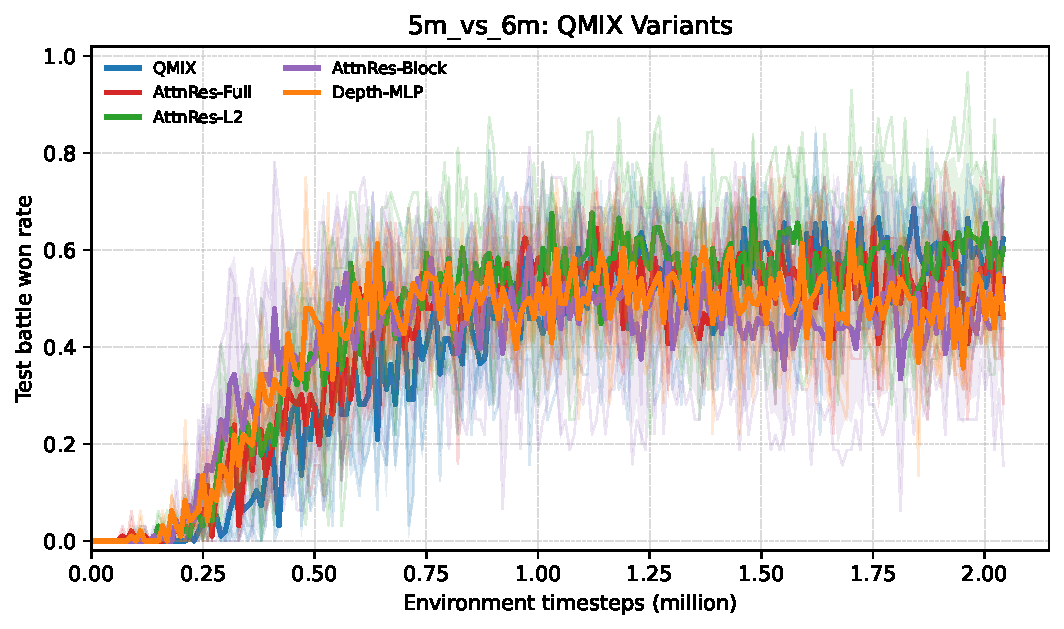
\includegraphics[width=0.92\linewidth]{figures/5m_vs_6m_qmix_win_curve.pdf}
  \caption{\code{5m\_vs\_6m} 上 QMIX 主实验变体的测试胜率学习曲线。曲线为 3 个 seeds 的均值，阴影表示标准差，浅色细线表示单个 seed。}
  \label{fig:5m-qmix-win-curve}
\end{figure}

\begin{figure}[H]
  \centering
  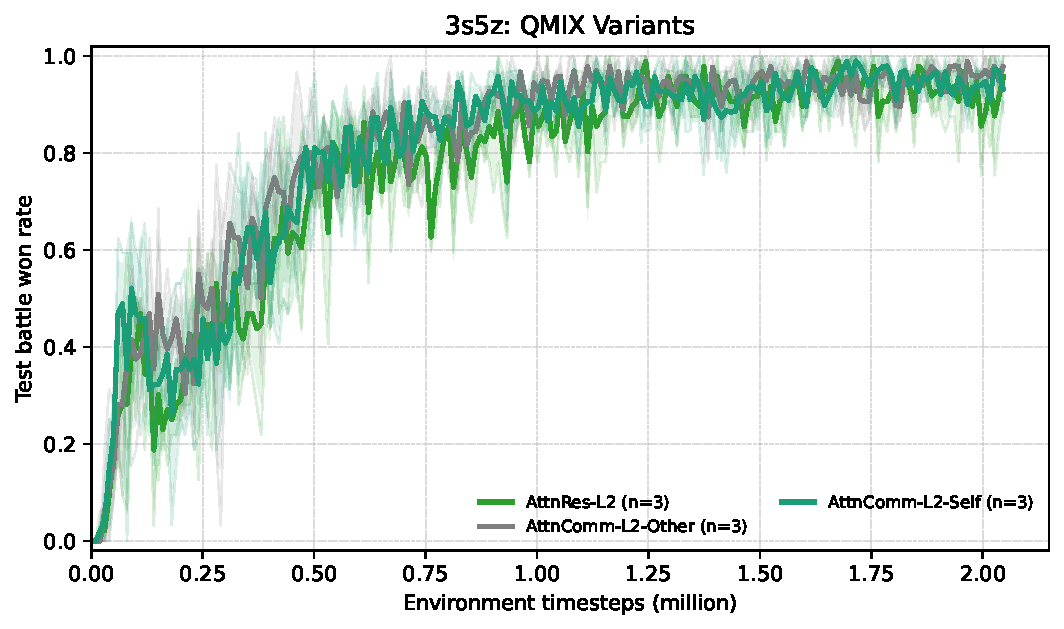
\includegraphics[width=0.92\linewidth]{figures/3s5z_qmix_win_curve.pdf}
  \caption{\code{3s5z} 上 QMIX 主实验变体的测试胜率学习曲线。曲线为 3 个 seeds 的均值，阴影表示标准差，浅色细线表示单个 seed。}
  \label{fig:3s5z-qmix-win-curve}
\end{figure}

\subsection{Depth-only Control 分析}

\code{qmix\_depth\_mlp} 在 \code{5m\_vs\_6m} 上的 final win rate 为 0.4583，低于 QMIX。
这说明单纯增加后处理网络深度并不能稳定带来收益。
该对照支持本文的分析重点：当前问题不是“网络加深一定有效”，而是需要判断选择性聚合机制是否真正适配 MARL agent。

\subsection{跨算法轻量 AttnRes-L2 验证}

\begin{table}[H]
  \centering
  \caption{跨算法轻量 AttnRes-L2 对照结果}
  \label{tab:cross-algorithm-results}
  \resizebox{\linewidth}{!}{
  \begin{tabular}{lllrrrrl}
    \toprule
    地图 & Baseline & Candidate & Paired Seeds & $\Delta$ Final Win & $\Delta$ Best Win & $\Delta$ AUC & 解释 \\
    \midrule
    \code{5m\_vs\_6m} & \code{iql} & \code{iql\_attnres\_l2} & 3 & +0.0833 & +0.1458 & +0.0455 & lightweight transfer 有正向信号 \\
    \code{5m\_vs\_6m} & \code{vdn} & \code{vdn\_attnres\_l2} & 3 & +0.0625 & +0.0104 & +0.0577 & AUC 提升但 seed 表现混合 \\
    \code{5m\_vs\_6m} & \code{qmix} & \code{qmix\_attnres\_l2} & 3 & -0.0208 & +0.0208 & +0.0567 & mixed or unstable \\
    \bottomrule
  \end{tabular}}
\end{table}


跨算法结果显示，AttnRes-L2 在 IQL、VDN 和 QMIX 三类 baseline 上均提高了平均 win-rate AUC，分别提升 0.0455、0.0577 和 0.0567。
这说明轻量化选择性聚合在学习过程中具有一定正向信号。
但是，final win rate 的表现并不一致：IQL 和 VDN 的平均 final win 分别提升 0.0833 和 0.0625，而 QMIX 的平均 final win 下降 0.0208。
从 paired seeds 看，VDN 的 final win 只在 1/3 seeds 上优于 baseline，AUC 在 2/3 seeds 上优于 baseline，因此更适合解释为 mixed or unstable，而不是稳定改进。
因此，本文仅将 AttnRes-L2 表述为具有 limited positive signal 的轻量化变体，不将其作为稳定优于既有价值分解方法的新算法。

\begin{table}[H]
  \centering
  \caption{\code{5m\_vs\_6m} 上 AttnRes-L2 的 paired seed delta。Delta 为 candidate 减 baseline。}
  \label{tab:paired-seed-delta}
  \resizebox{\linewidth}{!}{
  \begin{tabular}{llrrrrl}
    \toprule
    Baseline & Seed & Baseline Final & L2 Final & $\Delta$ Final & $\Delta$ AUC & Seed-level 判断 \\
    \midrule
    \code{iql} & 1 & 0.3750 & 0.3125 & -0.0625 & +0.0412 & mixed \\
    \code{iql} & 2 & 0.3750 & 0.6563 & +0.2813 & +0.0580 & candidate better \\
    \code{iql} & 3 & 0.4063 & 0.4375 & +0.0313 & +0.0372 & candidate better \\
    \midrule
    \code{vdn} & 1 & 0.6563 & 0.6250 & -0.0313 & -0.0585 & candidate worse \\
    \code{vdn} & 2 & 0.5625 & 0.7813 & +0.2188 & +0.1138 & candidate better \\
    \code{vdn} & 3 & 0.6563 & 0.6563 & +0.0000 & +0.1177 & mixed \\
    \midrule
    \code{qmix} & 1 & 0.7500 & 0.6875 & -0.0625 & +0.0887 & mixed \\
    \code{qmix} & 2 & 0.4375 & 0.6563 & +0.2188 & +0.1528 & candidate better \\
    \code{qmix} & 3 & 0.6875 & 0.4688 & -0.2188 & -0.0714 & candidate worse \\
    \bottomrule
  \end{tabular}}
\end{table}


表~\ref{tab:paired-seed-delta} 给出了 seed-level paired delta。
可以看到，IQL 的 3 个 seeds 均获得正向 AUC delta，但 final win 仍有一个 seed 下降；VDN 和 QMIX 则同时出现 candidate better、mixed 和 candidate worse。
这说明 AttnRes-L2 在学习过程中确实存在一定 AUC 信号，但最终胜率对 seed 和后端价值分解方法较敏感。

\begin{figure}[H]
  \centering
  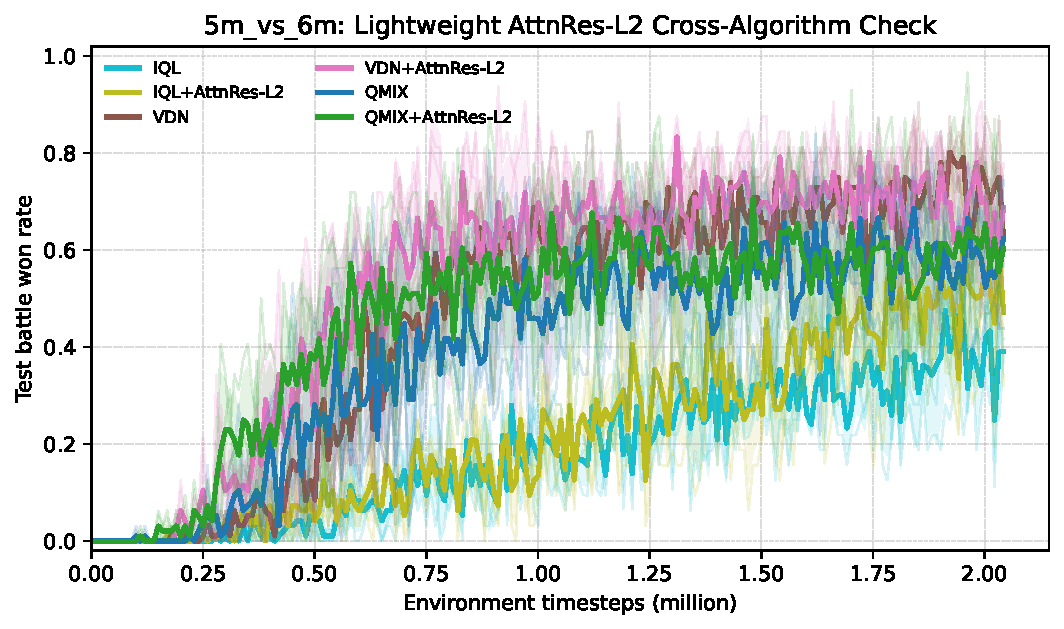
\includegraphics[width=0.92\linewidth]{figures/5m_vs_6m_cross_algorithm_win_curve.pdf}
  \caption{\code{5m\_vs\_6m} 上轻量 AttnRes-L2 的跨算法测试胜率曲线。曲线为 3 个 seeds 的均值，阴影表示标准差；图中包含 IQL、VDN、QMIX 及其 AttnRes-L2 变体。}
  \label{fig:cross-algorithm-win-curve}
\end{figure}

\subsection{Agent-wise Communication Extension}

前述结果表明，直接将 depth-wise Attention Residuals 插入浅层 recurrent agent 后并不能稳定形成 final win-rate 收益。
基于这一观察，本文进一步进行了一个小规模扩展实验：保持 QMIX learner、mixer 和动作选择器不变，只在 GRU hidden state 与 individual Q head 之间加入两层 agent-wise attention communication。
该扩展并不是替换 QMIX 算法，而是将 selective attention 从 depth dimension 转移到 agent dimension，用于检验跨智能体通信是否更符合 SMAC 的协同瓶颈。

\begin{table}[H]
  \centering
  \caption{\code{5m\_vs\_6m} 上 AttnComm-QMIX-L2 初步扩展结果（\(t_{\max}=5.0\)M）}
  \label{tab:attncomm-5m-extension}
  \resizebox{\linewidth}{!}{
  \begin{tabular}{lrrrrrr}
    \toprule
    变体 & Seeds & Final Win & Best Win & Win AUC & Wall Hours & 相对 QMIX AUC \(\Delta\) \\
    \midrule
    \code{qmix} & 3/3 & 0.5208 & 0.8021 & 0.4986 & 24.80 & -- \\
    \code{qmix\_attnres\_l2} & 3/3 & 0.5833 & 0.8021 & 0.5028 & 33.00 & +0.0043 \\
    \code{qmix\_attncomm\_l2\_other} & 3/3 & 0.6354 & 0.8542 & 0.5429 & 33.40 & +0.0444 \\
    \code{qmix\_attncomm\_l2\_self} & 3/3 & 0.5938 & 0.8646 & 0.5207 & 33.34 & +0.0222 \\
    \bottomrule
  \end{tabular}}
\end{table}


表~\ref{tab:attncomm-5m-extension} 给出了 \code{5m\_vs\_6m} 上 \(t_{\max}=5.0\)M 的完整 3-seed 初步结果。
在 3 个 paired seeds 上，\code{qmix\_attncomm\_l2\_other} 的 final win、best win 和 AUC 均高于 QMIX baseline，平均 final win 从 0.5208 提升到 0.6354，AUC 从 0.4986 提升到 0.5429，对应 final win \(+0.1146\)、AUC \(+0.0444\)。
\code{qmix\_attncomm\_l2\_self} 也取得正向均值提升，final win 和 AUC 分别提升 \(+0.0729\) 与 \(+0.0222\)，但幅度小于 other-only 版本。
从 paired comparison 看，other-only 版本在 final win 和 AUC 上均有 2/3 seeds 优于 baseline，self-inclusive 版本同样为 2/3 seeds 优于 baseline。
这说明 agent-wise communication attention 在当前设置下具有比 depth-wise hidden 后处理更直接的正向信号；同时，other-only 优于 self-inclusive 的现象也支持收益主要来自跨智能体信息聚合，而不只是额外的 self-attention 表示变换。

不过，该结果仍应谨慎解读。
首先，\code{qmix\_attnres\_l2} 在完整 3 seeds 后 final win 也高于 QMIX，但 AUC 增益仅为 \(+0.0043\)，best win 与 QMIX 持平，且 final win 标准差较大。
因此，完整 5M 对照并不支持“direct depth-wise transfer 已经稳定有效”的强结论，更适合表述为弱正向但高方差的结果。
其次，AttnComm 的平均 wall-clock time 约为 QMIX 的 1.35 倍，说明通信模块带来了额外成本，但该成本低于前文 heavy Full/Block AttnRes 的训练开销。
最后，当前 \code{3s5z} 的 AttnComm 运行仍不作为本文主结论依据，因此本文只将 \code{5m\_vs\_6m} 视为主要正向诊断结果，不声称跨地图稳定提升。

\begin{figure}[H]
  \centering
  \begin{subfigure}{0.48\linewidth}
    \centering
    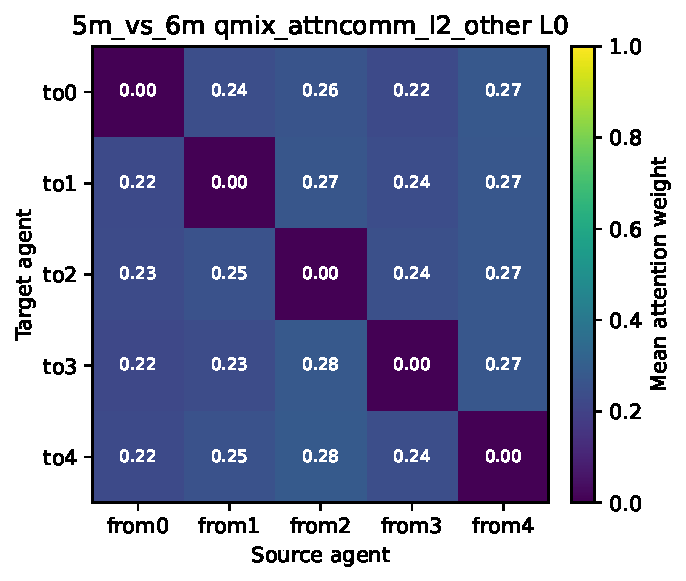
\includegraphics[width=\linewidth]{figures/5m_vs_6m_qmix_attncomm_l2_other_l0_attncomm_attention_heatmap.pdf}
    \caption{\code{other-only}, layer 0}
  \end{subfigure}
  \hfill
  \begin{subfigure}{0.48\linewidth}
    \centering
    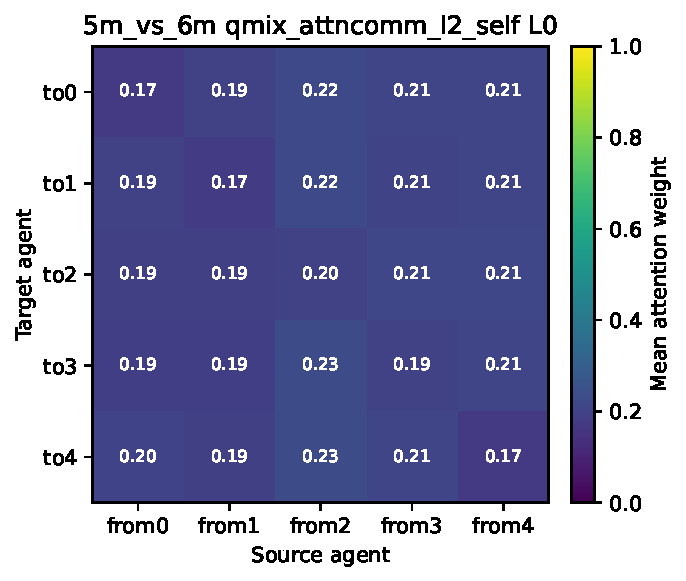
\includegraphics[width=\linewidth]{figures/5m_vs_6m_qmix_attncomm_l2_self_l0_attncomm_attention_heatmap.pdf}
    \caption{\code{self-inclusive}, layer 0}
  \end{subfigure}
  \caption{\code{5m\_vs\_6m} 上 AttnComm-L2 的 agent-to-agent attention heatmap。颜色表示跨 seeds 与日志点聚合后的平均 attention weight。}
  \label{fig:attncomm-heatmap}
\end{figure}

\subsection{训练效率分析}

训练时间显示，heavy variants 的成本显著高于 baseline。
在 \code{5m\_vs\_6m} 上，QMIX 平均训练时间约为 6.59 小时，而 \code{qmix\_attnres} 和 \code{qmix\_attnres\_block} 分别约为 15.14 小时和 13.97 小时。
\code{qmix\_attnres\_l2} 的成本约为 8.29 小时，明显低于重型版本，但仍高于 baseline。
在跨算法验证中，VDN+AttnRes-L2 的平均训练时间约为 VDN baseline 的 1.43 倍，进一步说明轻量化版本虽然比重型 AttnRes 更可控，但仍带来额外训练成本。
在 AttnComm 扩展实验中，两个通信变体的 wall-time ratio 约为 QMIX 的 1.35 倍。
这说明 agent-wise communication 相比原始 QMIX 仍有计算成本，但在当前 5M 训练设置下，其成本与收益之间呈现出比 heavy depth-wise AttnRes 更合理的折中。

\begin{figure}[H]
  \centering
  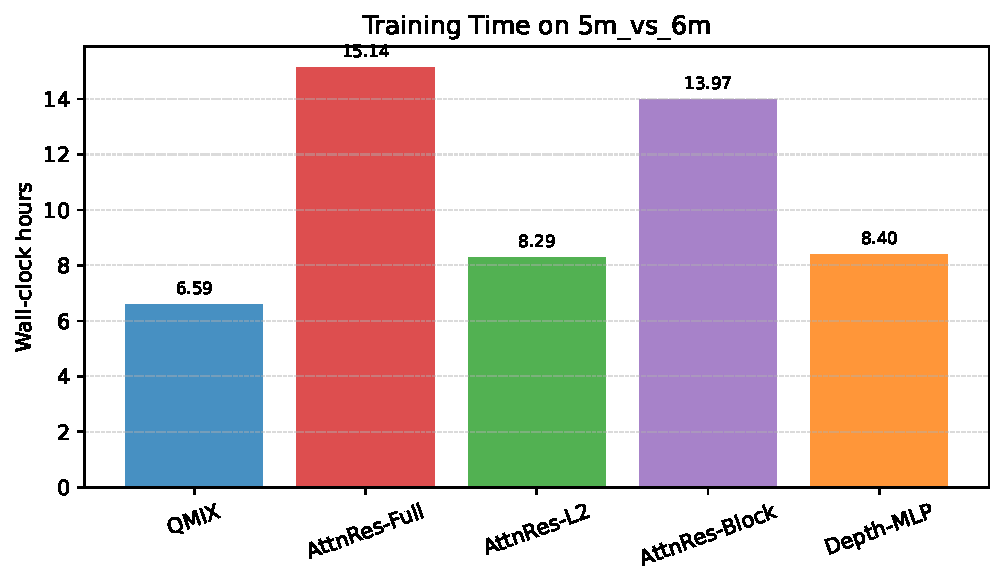
\includegraphics[width=0.82\linewidth]{figures/5m_vs_6m_wall_time_bar.pdf}
  \caption{\code{5m\_vs\_6m} 上各 QMIX 变体的平均训练墙钟时间。}
  \label{fig:wall-time-bar}
\end{figure}

\section{讨论}

\subsection{直接迁移不稳定的原因}

Attention Residuals 的原始目标是改善深层 LLM 中的 residual stream 信息选择。
而 PyMARL 中的 recurrent agent 较浅，主要瓶颈并不是跨层 residual dilution。
SMAC 中更关键的问题是多智能体协同、局部观测、探索路径和信用分配。
因此，将 AttnRes 作为 GRU hidden 的后处理模块可能存在结构错位。

\subsection{轻量化信号与局限}

AttnRes-L2 在 \code{5m\_vs\_6m} 的 AUC 和 best win 上有一定信号，在 IQL 上也显示出正向均值提升。
但这些收益没有稳定转化为 QMIX final win rate。
因此，当前结果更适合表述为“轻量化结构有潜力”，而不是“AttnRes 是稳定强算法”。

\subsection{后续方向：Agent-wise Attention Communication}

根据当前结果与师兄建议，下一阶段不应继续将 Kimi/AttnRes 模块硬塞到 GRU 后面，而应将 attention 用于智能体间通信。
可考虑如下结构：

\begin{equation}
  [h_1, h_2, \ldots, h_n]
  \rightarrow \mathrm{AgentWiseAttention}
  \rightarrow \mathrm{GatedResidualFusion}
  \rightarrow Q_i.
\end{equation}

该方向将 LLM 中“选择性聚合”的思想从 depth dimension 转移到 agent dimension，更符合 MARL 中跨智能体协同的任务瓶颈。

\begin{figure}[H]
  \centering
  \fbox{\parbox{0.86\linewidth}{
    \centering
    TODO: 绘制 Direct depth transfer 与 Agent-wise communication transfer 的概念对比图。
  }}
  \caption{从 depth-wise residual transfer 到 agent-wise communication transfer}
  \label{fig:attncomm}
\end{figure}

\subsection{方法局限}

当前研究仍存在以下局限：

\begin{itemize}
  \item seed 数量较少，统计显著性有限。
  \item VDN baseline 已补齐，但跨算法验证仍仅覆盖 \code{5m\_vs\_6m} 一张地图。
  \item 学习曲线图和 attention weight 分析尚未生成。
  \item 当前方法只修改 agent 侧，尚未探索 mixer 或 communication 结构。
\end{itemize}

\section{结论与未来工作}

本文研究了 Attention Residuals 从大语言模型到多智能体强化学习的迁移适配性。
实验结果表明，重型 Full/Block AttnRes 直接插入浅层 recurrent MARL agent 后并不能稳定提升性能，并且显著增加训练时间。
轻量化 AttnRes-L2 在部分指标上显示出 AUC 和 best-win 信号，完整 5M \code{5m\_vs\_6m} 对照中也获得了小幅 final-win 均值提升，但 AUC 增益很小且 seed 间方差较大。
因此，direct depth-wise transfer 并非完全无效，但其收益弱、不稳定，并不足以支撑稳定性能改进的结论。
进一步的 AttnComm-QMIX-L2 初步扩展实验显示，将 selective attention 放到 agent-wise communication 维度后，\code{5m\_vs\_6m} 上相对 QMIX baseline 出现了更明确的 final win 和 AUC 正向信号，其中 other-only communication 的平均提升更明显。

因此，当前结果不支持“Attention Residuals 可以直接作为浅层 MARL agent 后处理模块稳定提升性能”的强结论。
更合理的适配路径是将 selective attention 思想迁移到 agent-wise communication 中，用于建模智能体间协同关系。
从实验定位看，本文的主要价值在于给出一组可复现实验和适配性分析，而不是提出一个追求最优性能的新 MARL 算法。

当前实验已经足以支持上述谨慎结论，因此本文不将继续补跑 \code{3s5z}、扩展 AttnComm 到 IQL/VDN 或新增 hard map 作为定稿前的必要条件。
后续工作可以从以下方向增强证据：

\begin{itemize}
  \item 在更多 SMAC 地图上验证不同复杂度任务中的迁移表现，优先选择比 \code{3s5z} 更有区分度的中高难地图。
  \item 在 \code{5m\_vs\_6m} 上增加 paired seeds，进一步检验 AttnComm 与 AttnRes-L2 的 seed 稳定性。
  \item 在更有区分度的 SMAC 地图上继续验证 AttnComm 信号，而不仅依赖接近饱和的 \code{3s5z} sanity check。
  \item 在更多 SMAC 地图上比较 \code{qmix\_attncomm\_l2\_other} 与 \code{qmix\_attncomm\_l2\_self}，检验 other-only communication 信号是否稳定。
  \item 在 IQL 或 VDN 等其他后端上验证 AttnComm 是否仍具有类似趋势。
  \item 分析 communication attention weights 与 agent coordination 的关系。
  \item 增加统计显著性分析。
\end{itemize}


\bibliographystyle{plain}
\bibliography{references}

\appendix
\section{图表与材料清单}

\subsection{已生成图表}

\begin{itemize}
  \item \code{5m\_vs\_6m} QMIX variants win-rate learning curves。
  \item \code{3s5z} QMIX variants win-rate learning curves。
  \item \code{5m\_vs\_6m} IQL/VDN/QMIX cross-algorithm AttnRes-L2 learning curves。
  \item \code{3s5z} IQL/VDN/QMIX cross-algorithm AttnRes-L2 learning curves（follow-up 完成后生成）。
  \item \code{5m\_vs\_6m} QMIX variants training wall-clock bar chart。
  \item AttnRes-L2 attention heatmaps（基于记录 attention weights 的 seed4/5 runs）。
  \item PyMARL/QMIX 训练框架图。
  \item 原始 RNN agent、AttnRes-RNN agent、depth-only control 结构图。
\end{itemize}

\subsection{当前实验完整性}

当前预设实验中，QMIX 主线和 \code{5m\_vs\_6m} 跨算法验证均已补齐 3 个 seeds。
VDN baseline 新增 run 为：

\begin{itemize}
  \item \code{5m\_vs\_6m vdn seed1}: Sacred run 100。
  \item \code{5m\_vs\_6m vdn seed2}: Sacred run 101。
  \item \code{5m\_vs\_6m vdn seed3}: Sacred run 102。
\end{itemize}

重新汇总后，\code{marl\_transfer\_missing\_or\_partial.csv} 中无预设缺失项。
本轮 follow-up 使用 GPU 0/2/3/4/5/6 补充 \code{3s5z} 跨算法验证，并将核心 QMIX、AttnRes-L2 和 depth-only control 扩展到 seed4/5；Full/Block 仍保持 3 seeds。

\subsection{后续可扩展参考方向}

\begin{itemize}
  \item MARL 与 value decomposition：可继续补充 IQL、VDN、QMIX 之后的代表性改进方法。
  \item SMAC benchmark：可补充 SMACv2 或更复杂地图上的近期评测工作。
  \item Attention in MARL：可继续扩展 communication、graph attention 和 transformer-based MARL。
  \item Residual 与 Transformer：可补充更多跨层聚合、PreNorm 和深层网络稳定性研究。
  \item RL stability：可补充 off-policy value learning 和部分可观测 recurrent agents 的稳定性分析。
\end{itemize}


\end{document}
